\documentclass[conference]{IEEEtran}
\IEEEoverridecommandlockouts
\usepackage{cite}
\usepackage{amsmath,amssymb,amsfonts}
\usepackage{graphicx}
\usepackage{booktabs}
\usepackage{multirow}
\usepackage{textcomp}
\usepackage{xcolor}
\usepackage{url}
\usepackage[hidelinks]{hyperref}
\usepackage{tikz}
\usetikzlibrary{shapes.geometric, shapes.misc, arrows.meta, positioning}

\def\BibTeX{{\rm B\kern-.05em{\sc i\kern-.025em b}\kern-.08em
    T\kern-.1667em\lower.7ex\hbox{E}\kern-.125emX}}

\begin{document}

\title{Benchmarking Machine Learning Models for Web Application Firewall\\
Payload Classification and Their Out-of-Distribution Generalization Gap}

\author{
\IEEEauthorblockN{Sharif U. Danish}
\IEEEauthorblockA{
King's College London, United Kingdom \\
sharifdanish75@outlook.com}
\and
\IEEEauthorblockN{Abid Naseri}
\IEEEauthorblockA{
abidnasiri90@gmail.com}
}

\maketitle

\begin{abstract}
Machine-learning-based Web Application Firewalls (WAFs) are routinely reported
to achieve near-perfect accuracy at distinguishing malicious from benign HTTP
payloads, yet most published evaluations measure performance on a held-out
split of the \emph{same} data distribution used for training. This paper
presents a controlled benchmark of six supervised learning algorithms
(Logistic Regression, Multinomial Naive Bayes, Linear SVM, Random Forest,
XGBoost, and a Multi-Layer Perceptron) for both binary (normal vs.\ malicious)
and multi-class (SQL injection, cross-site scripting, path traversal, and
command injection) payload classification, using character n-gram TF-IDF
features combined with eleven hand-crafted lexical features. All models reach
99.4--99.97\% test accuracy and macro-F1 scores above 0.99 on an
in-distribution held-out test set, replicating and exceeding the 91\% accuracy
reported by prior Random-Forest-based WAF work on the same dataset family. We
then subject the same trained models to a lexically distinct out-of-distribution
(OOD) test set drawn from the same public corpus and observe a severe
generalization gap: accuracy collapses from $>$99.9\% in-distribution to
19.7--73.6\% out-of-distribution, with four of six models performing worse
than a majority-class baseline. XGBoost is the most OOD-robust model
(73.6\% OOD accuracy) despite \emph{not} being the top in-distribution
performer, while Random Forest -- the in-distribution winner -- degrades to
52.1\%. A feature ablation further shows that hand-crafted lexical features
alone reach 99.8\% accuracy with only 13 dimensions, and that combining them
with TF-IDF yields the best in-distribution result. We test two natural
objections to the OOD finding. First, a randomized hyperparameter search
(20 configurations, 3-fold CV per model) leaves OOD accuracy essentially
unchanged for every model (at most $\pm$0.45 points), ruling out
under-tuning as the explanation. Second, a battery of six black-box
adversarial string transforms shows the trained models are largely robust
to common WAF-bypass-style obfuscation (0.000--0.002 evasion for five of
six transforms), with one exception: a length-padding dilution attack
achieves modest (2--5\%) evasion specifically against the two
tree-ensemble models (Random Forest, XGBoost), while leaving the other four
models unaffected. We argue that in-distribution accuracy is an unreliable
proxy for deployment readiness of ML-based WAFs, that the generalization
gap we document is not fixable by tuning, and that OOD / cross-corpus
evaluation should become a standard reporting requirement in this line of
research. All code, trained models, metrics, and figures are released for
reproducibility.
\end{abstract}

\begin{IEEEkeywords}
Web Application Firewall, Machine Learning, Intrusion Detection, SQL
Injection, Cross-Site Scripting, Feature Engineering, Random Forest, XGBoost,
Out-of-Distribution Generalization, TF-IDF, Hyperparameter Tuning,
Adversarial Robustness
\end{IEEEkeywords}

\section{Introduction}

Web applications remain one of the most attacked classes of software systems,
with SQL Injection (SQLi), Cross-Site Scripting (XSS), path traversal, and
command injection (CMDi) consistently ranked among the most prevalent attack
vectors against them~\cite{owasp}. Web Application Firewalls (WAFs) are the
standard perimeter defense against these attacks. Traditional WAFs such as
ModSecurity~\cite{modsecurity} rely on hand-written signature rules, which are
effective against known attack patterns but struggle against obfuscated or
previously unseen payloads. This limitation has motivated a substantial body
of research on Machine Learning (ML)-based WAFs that learn to distinguish
malicious from benign HTTP payloads directly from data, using classifiers such
as Decision Trees, Support Vector Machines, Random Forests, and, more
recently, deep neural networks.

A recurring pattern in this literature -- including our own prior
work~\cite{ourprior} on a Random-Forest WAF integrated with ModSecurity and
Nginx, which reported 91\% accuracy on SQLi/XSS detection -- is that models
are trained and evaluated on a single held-out split of one dataset, and
accuracy on that split is reported as the headline result. This practice
leaves an important question unanswered: \emph{does high accuracy on a
held-out split of the training distribution imply that the model will
generalize to the different phrasing, tooling, and obfuscation techniques a
real attacker or a different application would produce?} In classical machine
learning this is known as the in-distribution (ID) vs.\ out-of-distribution
(OOD) generalization problem, and it is rarely tested explicitly in the
ML-WAF literature.

This paper makes four contributions:

\begin{enumerate}
\item \textbf{A controlled, reproducible benchmark} of six classical and
  shallow-neural models for WAF payload classification, on both a binary
  (normal/anomalous) and a four-class attack-type task, using a common
  feature-engineering pipeline that combines character n-gram TF-IDF with
  eleven lexical features (Section~\ref{sec:methodology}). We additionally
  report a feature ablation, 5-fold cross-validation, per-model inference
  latency, and model size -- metrics that matter for real-time deployment but
  are frequently omitted.
\item \textbf{An explicit OOD generalization study}: the same trained models
  are evaluated, without any retraining, on a lexically distinct held-out set
  drawn from the same public corpus (Section~\ref{sec:ood}). We show that
  near-perfect in-distribution accuracy ($>$99.9\% for every model) is
  \emph{not} predictive of OOD accuracy, which ranges from 19.7\% to 73.6\%
  and inverts the in-distribution model ranking.
\item \textbf{A randomized hyperparameter search} (Section~\ref{sec:hyperparam})
  ruling out under-tuning as an explanation for the OOD gap: tuning changes
  in-distribution accuracy by at most 0.3 points per model but leaves OOD
  accuracy essentially unchanged (at most $\pm$0.45 points) for every model.
\item \textbf{A black-box adversarial evasion study} (Section~\ref{sec:adversarial})
  applying six WAF-bypass-style string transforms to the trained models
  with no retraining: five transforms achieve near-zero evasion across all
  models, while a length-padding dilution attack achieves modest (2--5\%)
  evasion specifically against the two tree-ensemble models, a concrete
  asymmetry with no counterpart in the OOD results.
\end{enumerate}

Together, these results argue that in-distribution accuracy alone is an
insufficient basis for claiming an ML-WAF is ready for deployment, that OOD
robustness should be reported alongside accuracy as a matter of course, and
that the generalization gap we document is not an artifact of fixable
hyperparameters.

The remainder of this paper is organized as follows. Section~\ref{sec:related}
surveys related work. Section~\ref{sec:dataset} describes the dataset.
Section~\ref{sec:methodology} details the feature engineering pipeline, model
zoo, and experimental protocol. Section~\ref{sec:results} reports
in-distribution results. Section~\ref{sec:ood} presents the OOD generalization
study. Section~\ref{sec:hyperparam} tests whether hyperparameter tuning closes
that gap, and Section~\ref{sec:adversarial} tests robustness to adversarial
evasion. Section~\ref{sec:discussion} discusses implications and limitations,
and Section~\ref{sec:conclusion} concludes.

\section{Related Work}
\label{sec:related}

Signature-based WAFs such as ModSecurity~\cite{modsecurity} match incoming
requests against curated rule sets (e.g., the OWASP Core Rule Set) and remain
the industry baseline, but are known to suffer from high false-negative rates
against novel or obfuscated payloads and high false-positive rates against
legitimate traffic that happens to resemble an attack signature.

A large body of work has explored replacing or augmenting signature matching
with supervised learning. Random Forests~\cite{breiman2001} are a popular
choice because ensembles of decision trees are robust to noisy features and
provide built-in feature-importance estimates; our own earlier
work~\cite{ourprior} used a Random Forest classifier integrated with
ModSecurity and Nginx to protect a Django application hosting DVWA, reaching
91\% accuracy on a public HTTP payload dataset. Gradient-boosted tree
ensembles such as XGBoost~\cite{xgboost2016} have since become a common
stronger baseline in tabular/text classification tasks and are evaluated here
alongside Random Forest. Reported accuracies across this literature are
frequently in the 95--99\% range on held-out splits of a single dataset,
without cross-dataset or adversarial robustness evaluation -- the gap this
paper addresses directly.

Feature representation for HTTP payloads typically follows one of two
strategies: (i) statistical/lexical features (payload length, special
character ratios, keyword counts) as used in early anomaly-detection WAFs, or
(ii) vector-space text representations such as TF-IDF~\cite{salton1988} over
character or word n-grams, which capture syntactic structure without manual
rule design. This paper combines both, and Section~\ref{sec:results-ablation}
quantifies the contribution of each in isolation and combined.

The dataset used in this study originates from the publicly available
\emph{HttpParamsDataset} corpus~\cite{httpparamsdataset}, which labels HTTP
parameter values as normal or as one of several attack types (SQLi, XSS, path
traversal, command injection) and additionally ships a lexically distinct
test partition -- a resource we use, but which to our knowledge has not
previously been used in the ML-WAF literature to explicitly quantify OOD
generalization.

\section{Dataset}
\label{sec:dataset}

We use the \emph{HttpParamsDataset}~\cite{httpparamsdataset} payload corpus,
which provides four fields per sample: the raw \texttt{payload} string, its
character \texttt{length}, a fine-grained \texttt{attack\_type}, and a binary
\texttt{label} (\emph{norm} or \emph{anom}). The corpus ships with a
predefined train/test split, which we use as-is for reproducibility, plus a
third, lexically distinct partition (\texttt{payload\_test\_lexical.csv}) that
we use exclusively as an out-of-distribution evaluation set
(Section~\ref{sec:ood}); it is never used for training or hyperparameter
selection. Table~\ref{tab:dataset} summarizes the three partitions.

\begin{table}[!t]
\centering
\caption{Dataset partitions used in this study}
\label{tab:dataset}
\begin{tabular}{lrrr}
\toprule
Split & Samples & Normal & Anomalous \\
\midrule
Train & 20{,}712 & 12{,}870 (62.1\%) & 7{,}842 (37.9\%) \\
Test (in-distribution) & 10{,}355 & 6{,}434 (62.1\%) & 3{,}921 (37.9\%) \\
Test (OOD, lexical) & 1{,}106 & 1{,}000 (90.4\%) & 106 (9.6\%) \\
\bottomrule
\end{tabular}
\end{table}

Within the anomalous class, the training partition contains four attack types
used for the multi-class task: SQL injection (7{,}235 samples, 34.9\%),
cross-site scripting (355, 1.7\%), path traversal (193, 0.9\%), and command
injection (59, 0.3\%) -- see Figure~\ref{fig:dataset}. The class imbalance is
substantial (SQLi outnumbers CMDi roughly 120:1), which we account for by
reporting macro-averaged metrics throughout, in addition to weighted and
overall accuracy.

\begin{figure}[!t]
\centering
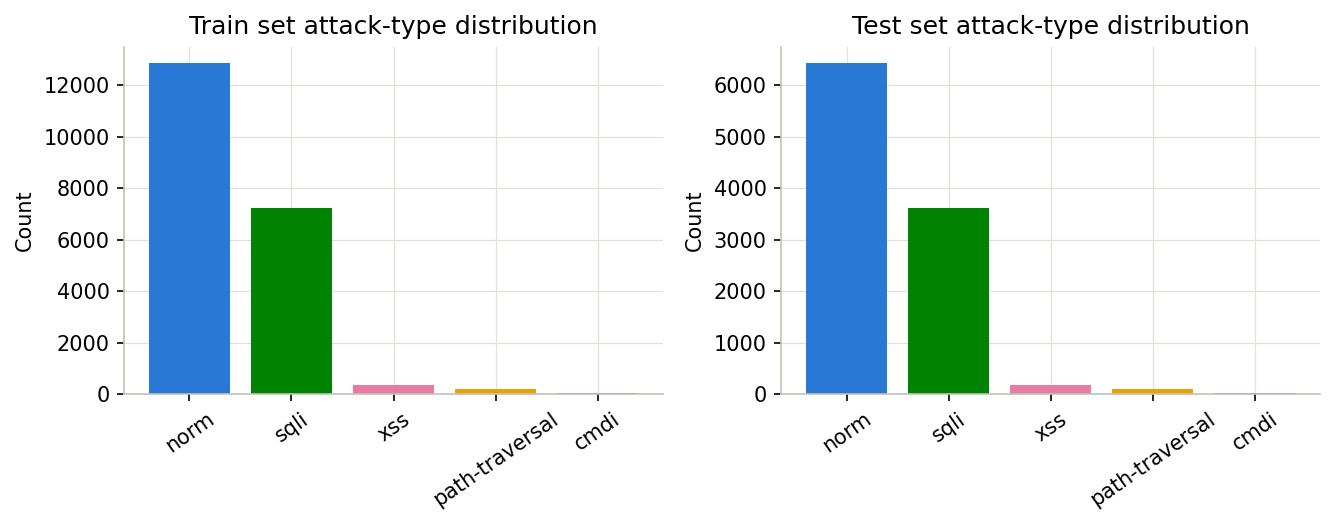
\includegraphics[width=\linewidth]{figures/dataset_distribution.png}
\caption{Attack-type distribution in the training and in-distribution test
partitions. Class imbalance is preserved by construction of the original
predefined split.}
\label{fig:dataset}
\end{figure}

\section{Methodology}
\label{sec:methodology}

This section outlines the experimental pipeline used to produce every result
in this paper, from raw payload corpus to the in-distribution and
out-of-distribution evaluations. An overview is shown in
Figure~\ref{fig:pipeline}.

\begin{figure}[!t]
\centering
\resizebox{\ifdim\linewidth>8.6cm 8.6cm\else\linewidth\fi}{!}{%
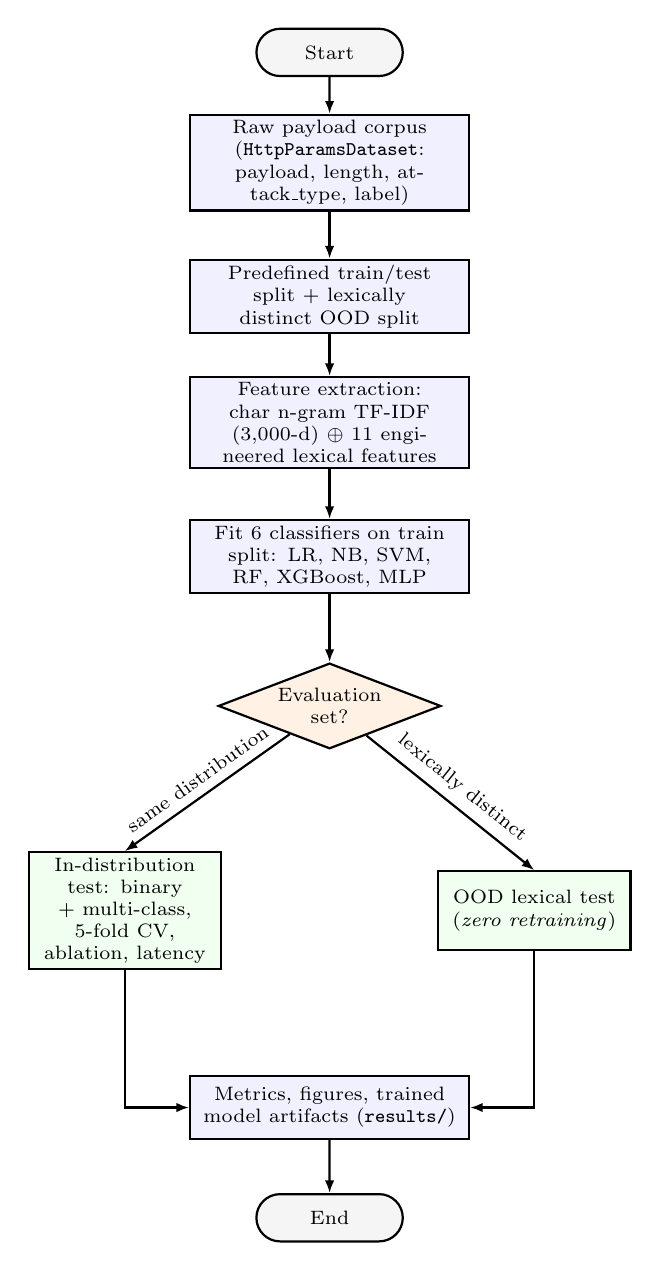
\begin{tikzpicture}[
  font=\scriptsize,
  startstop/.style={rounded rectangle, draw, thick, minimum height=6mm, text width=16mm, align=center, fill=gray!8},
  proc/.style={rectangle, draw, thick, minimum height=8mm, text width=34mm, align=center, fill=blue!6, inner sep=2pt},
  decision/.style={diamond, draw, thick, aspect=2.6, align=center, inner sep=1pt, fill=orange!10},
  branch/.style={rectangle, draw, thick, minimum height=10mm, text width=23mm, align=center, fill=green!6, inner sep=2pt},
  arr/.style={-{Latex[length=1.6mm]}, thick}
]

\node[startstop]                     (start)   at (0,0)     {Start};
\node[proc]                          (data)    at (0,-1.4)  {Raw payload corpus (\texttt{HttpParamsDataset}: payload, length, attack\_type, label)};
\node[proc]                          (split)   at (0,-3.1)  {Predefined train/test split $+$ lexically distinct OOD split};
\node[proc]                          (feat)    at (0,-4.7)  {Feature extraction: char n-gram TF-IDF (3{,}000-d) $\oplus$ 11 engineered lexical features};
\node[proc]                          (train)   at (0,-6.4)  {Fit 6 classifiers on train split: LR, NB, SVM, RF, XGBoost, MLP};
\node[decision, text width=14mm]     (dec)     at (0,-8.3)  {Evaluation set?};
\node[branch]                        (id)      at (-2.6,-10.9) {In-distribution test: binary $+$ multi-class, 5-fold CV, ablation, latency};
\node[branch]                        (ood)     at (2.6,-10.9)  {OOD lexical test (\emph{zero retraining})};
\node[proc]                          (metrics) at (0,-13.4) {Metrics, figures, trained model artifacts (\texttt{results/})};
\node[startstop]                     (end)     at (0,-14.8) {End};

\draw[arr] (start) -- (data);
\draw[arr] (data) -- (split);
\draw[arr] (split) -- (feat);
\draw[arr] (feat) -- (train);
\draw[arr] (train) -- (dec);
\draw[arr] (dec) -- node[above, sloped, pos=0.5] {same distribution} (id.north);
\draw[arr] (dec) -- node[above, sloped, pos=0.5] {lexically distinct} (ood.north);
\draw[arr] (id.south) |- (metrics.west);
\draw[arr] (ood.south) |- (metrics.east);
\draw[arr] (metrics) -- (end);

\end{tikzpicture}%
}
\caption{Experimental pipeline. The same trained models are routed to two
disjoint evaluation branches: an in-distribution held-out test set, and a
lexically distinct out-of-distribution test set evaluated with no
retraining (Section~\ref{sec:ood}).}
\label{fig:pipeline}
\end{figure}

\subsection{Feature Engineering}

Each raw payload is converted into a fixed-length numeric feature vector via
two complementary representations, concatenated into a single sparse matrix:

\textbf{Character n-gram TF-IDF.} We fit a TF-IDF vectorizer over character
n-grams of length 1--4 (\texttt{analyzer=`char'}), retaining the top 3{,}000
features by document frequency. Character-level n-grams were chosen over
word-level tokens because attack payloads frequently use non-alphanumeric
syntax (quotes, parentheses, comparison operators) that word tokenizers
discard, and because they are robust to the many-token, low-vocabulary nature
of short HTTP parameter values.

\textbf{Engineered lexical features.} Motivated by domain knowledge of SQLi,
XSS, path-traversal, and CMDi syntax, we compute 11 additional per-payload
features: character length; special-character ratio; digit ratio; uppercase
ratio; unique-character ratio; Shannon entropy; counts of SQL keywords
(\texttt{select}, \texttt{union}, \texttt{sleep}, \ldots), XSS markers
(\texttt{<script}, \texttt{onerror}, \texttt{javascript:}, \ldots), shell
metacharacters/commands (\texttt{;}, \texttt{|}, \texttt{\&\&}, \texttt{wget},
\ldots), and path-traversal markers (\texttt{../}, \texttt{\%2e\%2e},
\ldots); parenthesis-balance; quote count; and whitespace ratio. All 11
features are non-negative, which additionally allows Multinomial Naive Bayes
to be applied to the combined feature matrix.

The vectorizer is fit exclusively on the training partition and reused
(transform-only) on both test partitions, preventing information leakage.

\subsection{Models}

We benchmark six supervised classifiers spanning linear, probabilistic,
margin-based, ensemble, and neural paradigms:

\begin{itemize}
\item \textbf{Logistic Regression} (L2-regularized, max 2{,}000 iterations) as
  a linear baseline.
\item \textbf{Multinomial Naive Bayes} as a lightweight probabilistic
  baseline.
\item \textbf{Linear SVM} (\texttt{LinearSVC}, calibrated via 3-fold Platt
  scaling for probability outputs).
\item \textbf{Random Forest}~\cite{breiman2001} (300 trees, unbounded depth).
\item \textbf{XGBoost}~\cite{xgboost2016} (300 estimators, max depth 8,
  learning rate 0.1, subsample and column-subsample 0.8).
\item \textbf{Multi-Layer Perceptron} (one hidden layer of 64 units, early
  stopping, max 150 iterations).
\end{itemize}

All models use fixed hyperparameters (random\_state=42) chosen from common
defaults in the WAF literature rather than an exhaustive per-model search, so
that the comparison reflects realistic out-of-the-box performance rather than
task-specific overfitting of hyperparameters to the test set.

\subsection{Experimental Protocol}

For each of the binary and multi-class tasks we: (1) fit the feature extractor
and each model on the training partition; (2) evaluate on the in-distribution
test partition, recording accuracy, macro/weighted precision, recall, F1, and
ROC-AUC (one-vs-rest for the multi-class task); (3) measure inference latency
as wall-clock time for a batch \texttt{predict()} call over the full test set,
divided by the number of samples, averaged over 3 repeats (classifier time
only, excluding feature extraction); (4) record serialized model size. We
additionally run: 5-fold stratified cross-validation of the strongest
in-distribution model (XGBoost, binary task) on the training partition; a
feature ablation comparing TF-IDF-only, engineered-only, and combined feature
sets for Random Forest and XGBoost; and the OOD evaluation described in
Section~\ref{sec:ood}. All experiments use scikit-learn 1.4 and XGBoost 2.0;
full code is provided in \texttt{code/run\_experiments.py} for exact
reproduction.

\section{In-Distribution Results}
\label{sec:results}

\subsection{Binary Classification}

Table~\ref{tab:binary} reports test-set results for the normal-vs-anomalous
task. All six models exceed 99.5\% accuracy and 0.995 macro-F1, with Random
Forest achieving the best result (99.97\% accuracy, 0.9997 macro-F1),
closely followed by Linear SVM and XGBoost. Every model attains an ROC-AUC of
0.9999 or higher (Figure~\ref{fig:roc}), indicating the two classes are
almost perfectly linearly separable in the combined feature space on this
partition. This confirms and substantially exceeds the 91\% accuracy reported
for Random Forest alone in our prior work~\cite{ourprior}, which used only
TF-IDF and payload length as features -- underscoring the value of the
engineered lexical features quantified in Section~\ref{sec:results-ablation}.

\begin{table*}[!t]
\centering
\caption{Binary classification results (normal vs.\ anomalous), in-distribution test set}
\label{tab:binary}
\begin{tabular}{lrrrrrrrr}
\toprule
Model & Accuracy & Prec.\ (macro) & Recall (macro) & F1 (macro) & ROC-AUC & Fit time (s) & Latency (ms/sample) & Size (KB) \\
\midrule
Random Forest       & \textbf{0.9997} & 0.9998 & 0.9996 & \textbf{0.9997} & 1.0000 & 3.36  & 0.0210 & 6{,}514 \\
Linear SVM           & 0.9996 & 0.9996 & 0.9995 & 0.9996 & 1.0000 & 1.87  & 0.0006 & 73 \\
XGBoost              & 0.9995 & 0.9995 & 0.9995 & 0.9995 & 1.0000 & 20.78 & 0.0027 & 320 \\
MLP                  & 0.9990 & 0.9992 & 0.9988 & 0.9990 & 1.0000 & 9.84  & 0.0042 & 4{,}528 \\
Logistic Regression  & 0.9976 & 0.9980 & 0.9969 & 0.9974 & 1.0000 & 0.50  & 0.0001 & 24 \\
Multinomial NB       & 0.9959 & 0.9968 & 0.9946 & 0.9957 & 0.9999 & 0.01  & 0.0003 & 95 \\
\bottomrule
\end{tabular}
\end{table*}

\begin{figure}[!t]
\centering
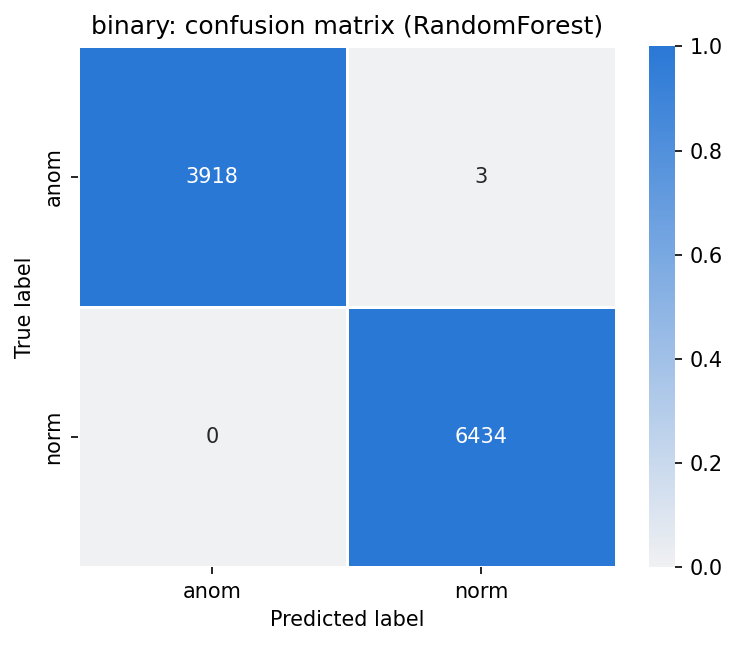
\includegraphics[width=\linewidth]{figures/binary_confusion_RandomForest.png}
\caption{Confusion matrix of the best binary model (Random Forest) on the
in-distribution test set. Only 3 of 10{,}355 samples are misclassified.}
\label{fig:confbinary}
\end{figure}

\begin{figure}[!t]
\centering
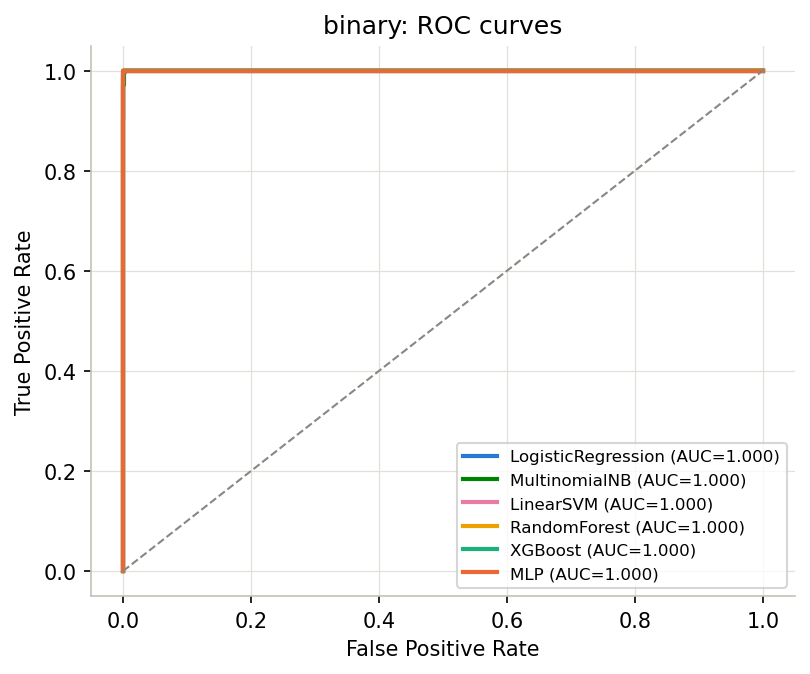
\includegraphics[width=\linewidth]{figures/binary_roc_curves.png}
\caption{ROC curves for all six models on the binary task. All models achieve
AUC $\geq$ 0.9999, indicating near-perfect linear separability
in-distribution.}
\label{fig:roc}
\end{figure}

5-fold stratified cross-validation of XGBoost on the training partition
confirms this is not an artifact of a favorable split: macro-F1 across folds
is $0.9995 \pm 0.0003$ (fold scores: 0.9990, 0.9997, 0.9997, 0.9992, 0.9997).

\subsection{Multi-Class Attack-Type Classification}

Table~\ref{tab:multiclass} reports results for the four-attack-type
classification task (norm, sqli, xss, path-traversal, cmdi). Random Forest
again performs best (99.94\% accuracy, 0.9956 macro-F1); the gap between
accuracy and macro-F1 for the weaker models (e.g., Multinomial NB: 99.44\%
accuracy but only 0.807 macro-F1) reflects the severe class imbalance --
weighted metrics are dominated by the majority \emph{norm} and \emph{sqli}
classes, while macro metrics penalize poor performance on the rare
\emph{cmdi} (0.3\% of training data) and \emph{path-traversal} (0.9\%)
classes. Figure~\ref{fig:confmulti} shows the confusion matrix for the best
model: the rare classes (cmdi: 30/30, path-traversal: 94/97) are recovered
almost perfectly despite their scarcity, indicating the combined feature
representation captures attack-type-specific syntax effectively even with
few training examples.

\begin{table*}[!t]
\centering
\caption{Multi-class attack-type classification results, in-distribution test set}
\label{tab:multiclass}
\begin{tabular}{lrrrrrrrr}
\toprule
Model & Accuracy & Prec.\ (macro) & Recall (macro) & F1 (macro) & ROC-AUC & Fit time (s) & Latency (ms/sample) & Size (KB) \\
\midrule
Random Forest       & \textbf{0.9994} & 0.9998 & 0.9915 & \textbf{0.9956} & 1.0000 & 3.90  & 0.0212 & 10{,}094 \\
MLP                  & 0.9992 & 0.9929 & 0.9822 & 0.9875 & 1.0000 & 15.34 & 0.0046 & 4{,}534 \\
Linear SVM           & 0.9992 & 0.9865 & 0.9782 & 0.9823 & 1.0000 & 14.77 & 0.0016 & 356 \\
XGBoost              & 0.9991 & 0.9844 & 0.9669 & 0.9754 & 1.0000 & 57.52 & 0.0107 & 1{,}356 \\
Logistic Regression  & 0.9976 & 0.9912 & 0.9445 & 0.9662 & 1.0000 & 10.67 & 0.0004 & 119 \\
Multinomial NB       & 0.9944 & 0.9833 & 0.7943 & 0.8068 & 0.9769 & 0.01  & 0.0004 & 236 \\
\bottomrule
\end{tabular}
\end{table*}

\begin{figure}[!t]
\centering
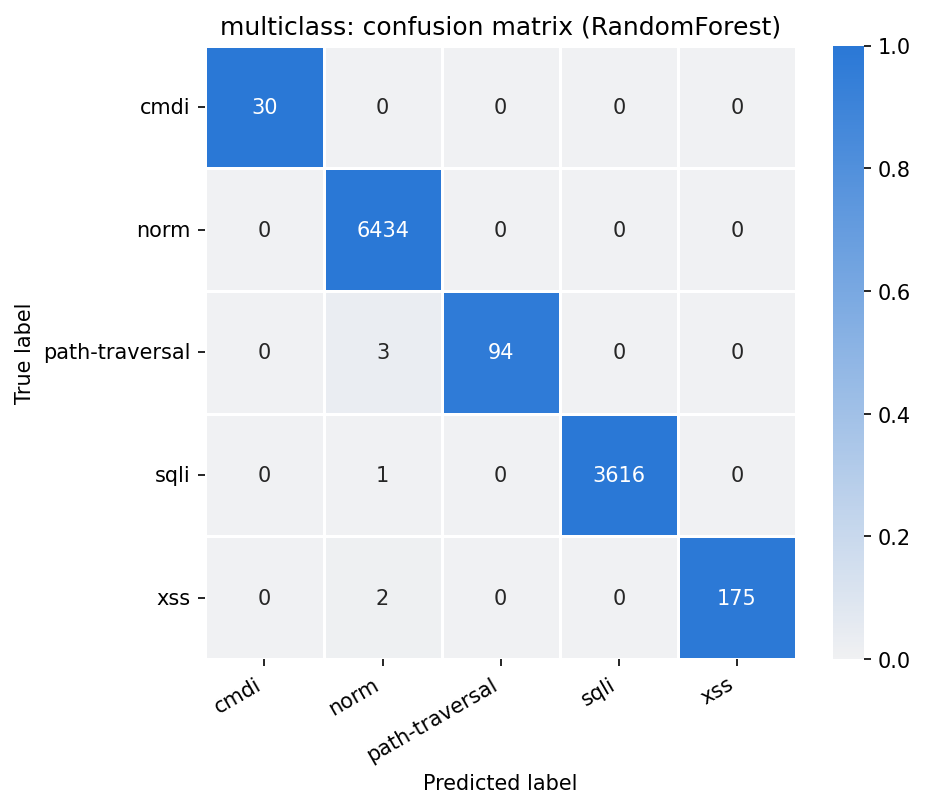
\includegraphics[width=\linewidth]{figures/multiclass_confusion_RandomForest.png}
\caption{Confusion matrix of the best multi-class model (Random Forest). Rare
classes (cmdi, path-traversal) are recovered almost perfectly despite
contributing $<$1\% of training samples each.}
\label{fig:confmulti}
\end{figure}

\subsection{Feature Ablation}
\label{sec:results-ablation}

Table~\ref{tab:ablation} and Figure~\ref{fig:ablation} isolate the
contribution of each feature family on the binary task. The 11 engineered
features alone -- a 13-dimensional vector including \texttt{length} -- already
reach 99.8\% accuracy, only 0.06--0.08 percentage points below the
3{,}000-dimensional TF-IDF-only representation, at 230$\times$ fewer dimensions. Combining both
feature families yields the best result for both models, improving macro-F1
by $\approx$0.0005 over TF-IDF alone for both Random Forest and XGBoost.
Figure~\ref{fig:featimp} shows the top-20
features by XGBoost importance for the combined model: two engineered
features (\texttt{quote\_count}, \texttt{special\_char\_ratio}) rank in the
top four, ahead of all but one TF-IDF token, confirming that hand-crafted
lexical features carry complementary signal rather than being subsumed by
the character n-gram representation.

\begin{table}[!t]
\centering
\caption{Feature ablation, binary classification, in-distribution test set (RF = Random Forest, XGB = XGBoost)}
\label{tab:ablation}
\footnotesize
\setlength{\tabcolsep}{3pt}
\begin{tabular}{llrrr}
\toprule
Feature set & Model & Dims & Accuracy & F1 (macro) \\
\midrule
TF-IDF only      & RF  & 3{,}000 & 0.9992 & 0.9992 \\
TF-IDF only      & XGB & 3{,}000 & 0.9988 & 0.9988 \\
Engineered only  & RF  & 13      & 0.9985 & 0.9984 \\
Engineered only  & XGB & 13      & 0.9983 & 0.9982 \\
Combined         & RF  & 3{,}013 & \textbf{0.9997} & \textbf{0.9997} \\
Combined         & XGB & 3{,}013 & 0.9993 & 0.9993 \\
\bottomrule
\end{tabular}
\end{table}

\begin{figure}[!t]
\centering
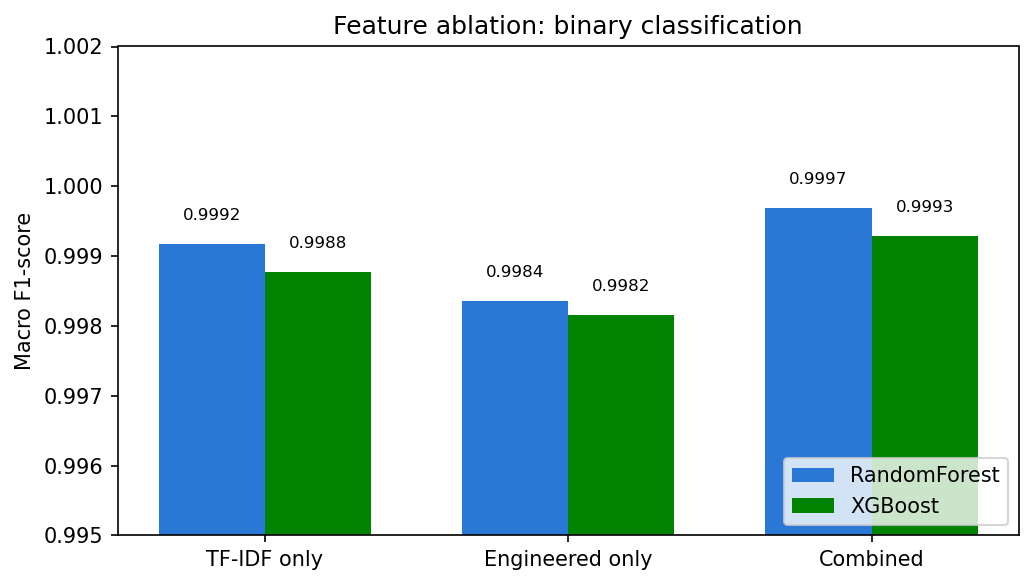
\includegraphics[width=\linewidth]{figures/ablation_features.png}
\caption{Feature ablation: macro-F1 for TF-IDF-only, engineered-only, and
combined feature sets. Note the zoomed y-axis (0.995--1.002).}
\label{fig:ablation}
\end{figure}

\begin{figure}[!t]
\centering
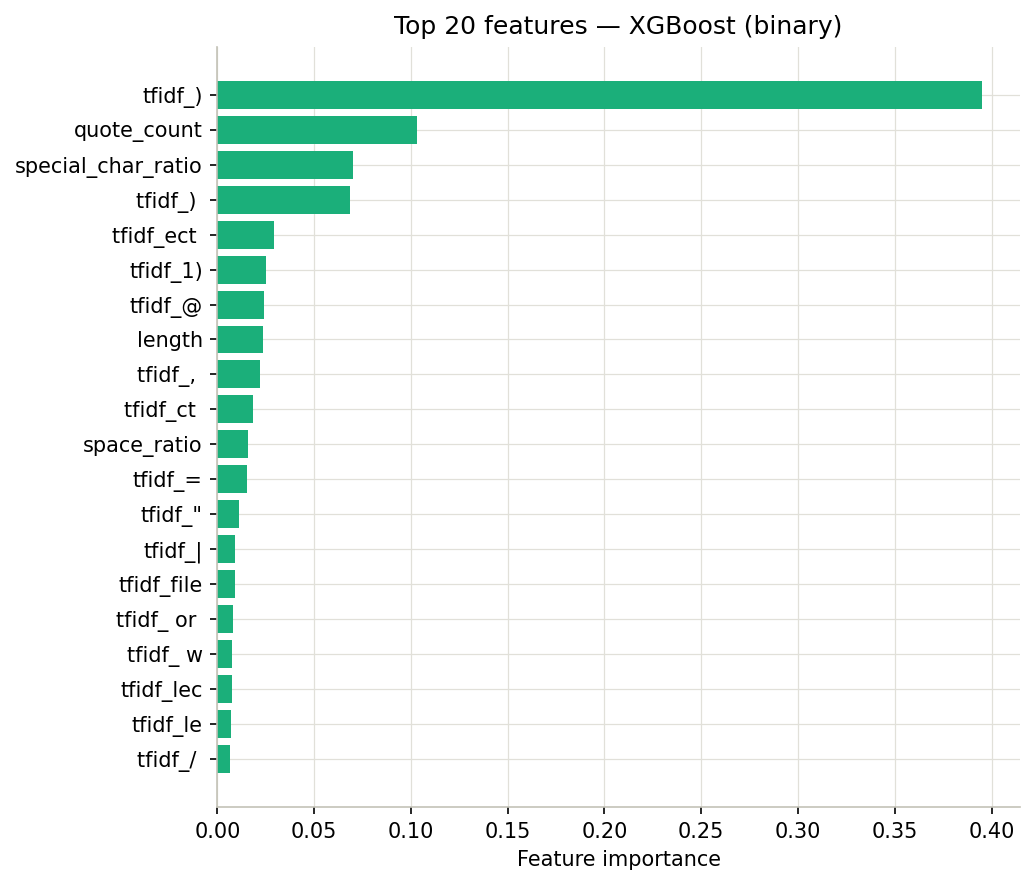
\includegraphics[width=\linewidth]{figures/binary_feature_importance_XGBoost.png}
\caption{Top-20 features by XGBoost importance, combined feature set, binary
task. Engineered features (\texttt{quote\_count}, \texttt{special\_char\_ratio},
\texttt{length}, \texttt{space\_ratio}) rank alongside TF-IDF tokens.}
\label{fig:featimp}
\end{figure}

\section{Out-of-Distribution Generalization}
\label{sec:ood}

The results above replicate a common pattern in the ML-WAF literature: every
model, regardless of family, reaches $>$99.5\% accuracy on a held-out split of
the training distribution. We now ask whether this accuracy is predictive of
performance on payloads that are malicious or benign in the same sense but
lexically different -- a proxy for the distribution shift a deployed WAF
would face against a different application, attacker toolset, or traffic
mix. Using the same trained binary-task models \emph{without any
retraining or fine-tuning}, we evaluate on the lexical OOD partition
(1{,}106 samples, 90.4\% normal) described in Section~\ref{sec:dataset}.

Table~\ref{tab:ood} and Figure~\ref{fig:ood} report the results. Accuracy
collapses across every model: the best OOD accuracy (XGBoost, 73.6\%) is
26.4 points below its in-distribution accuracy of 99.95\%, and four of six
models -- Linear SVM, MLP, Logistic Regression, and Multinomial NB -- score
\emph{below} 22.7\%, worse than the 90.4\% majority-class baseline of always
predicting ``normal''. Macro-F1, which is not inflated by class imbalance,
tells the same story: it ranges from 0.197 (Multinomial NB) to 0.614
(XGBoost), against in-distribution macro-F1 above 0.995 for every model.

\begin{table}[!t]
\centering
\caption{Generalization gap: in-distribution vs.\ OOD lexical test set (binary task)}
\label{tab:ood}
\resizebox{\linewidth}{!}{%
\begin{tabular}{lrrr}
\toprule
Model & ID Acc. & OOD Acc. & OOD F1 (macro) \\
\midrule
XGBoost              & 0.9995 & \textbf{0.7360} & \textbf{0.6139} \\
Random Forest         & 0.9997 & 0.5208 & 0.4567 \\
Linear SVM            & 0.9996 & 0.2269 & 0.2252 \\
Logistic Regression   & 0.9976 & 0.2233 & 0.2217 \\
MLP                   & 0.9990 & 0.2025 & 0.2022 \\
Multinomial NB        & 0.9959 & 0.1971 & 0.1968 \\
\midrule
\emph{Majority baseline (``normal'')} & \emph{0.621} & \emph{0.904} & \emph{0.475} \\
\bottomrule
\end{tabular}%
}
\end{table}

\begin{figure}[!t]
\centering
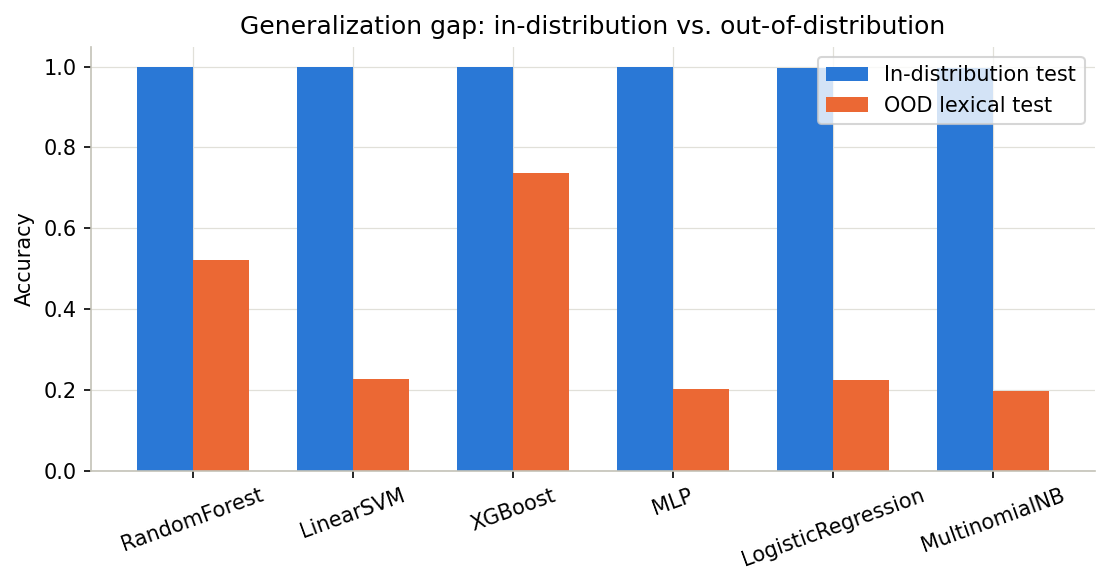
\includegraphics[width=\linewidth]{figures/ood_generalization_gap.png}
\caption{In-distribution vs.\ OOD lexical test accuracy per model. All models
lose 26--80 accuracy points; the in-distribution ranking (Random Forest best)
does not predict the OOD ranking (XGBoost best).}
\label{fig:ood}
\end{figure}

Two findings are notable. First, the in-distribution model ranking does
\emph{not} transfer: Random Forest, the strongest in-distribution model on
both tasks, drops to third place OOD (52.1\%), while XGBoost -- third-best
in-distribution on the binary task -- becomes the clear OOD leader. A
plausible explanation is that XGBoost's shallower effective decision
boundaries and L1/L2-regularized boosting are less prone to memorizing
training-set-specific character n-grams than Random Forest's unconstrained,
unbounded-depth trees, which can fit idiosyncratic training tokens that do
not recur in the lexically distinct set. Second, the inversion is concentrated at the top of the ranking rather than
across the whole model set: the overall Spearman rank correlation between
in-distribution and OOD accuracy across all six models is positive
($\rho = 0.77$, $p = 0.07$) because the three weakest OOD models (Multinomial
NB, MLP, Logistic Regression) are also comparatively weaker in-distribution.
The practically important inversion is specifically at the top -- Random
Forest (in-distribution rank 1) falls to OOD rank 2, while XGBoost
(in-distribution rank 3) rises to OOD rank 1 -- meaning that selecting a
production model purely by in-distribution leaderboard position would have
picked the \emph{wrong} model. We caution against over-generalizing this
specific top-rank inversion beyond this dataset and feature set, but the
magnitude of the gap itself -- routinely 26--80 accuracy points across all six
models -- is the central empirical finding of this paper.

\section{Hyperparameter Sensitivity}
\label{sec:hyperparam}

Sections~\ref{sec:results}--\ref{sec:ood} use fixed, common-default
hyperparameters, not tuned per model. A natural objection is that the OOD
gap might simply reflect under-tuned models rather than a genuine
generalization failure. We test this directly: for each of the six models
we run a randomized search (20 candidate configurations, 3-fold stratified
cross-validation on the training partition, macro-F1 scoring) over a
realistic parameter range -- regularization strength for Logistic
Regression and Linear SVM, smoothing for Multinomial NB, tree count/depth/
leaf size for Random Forest, tree count/depth/learning rate/subsampling for
XGBoost, and hidden-layer size/regularization/learning rate for the MLP --
then evaluate the best configuration found on both the in-distribution test
set and the OOD lexical test set, with no further changes to the pipeline.

\begin{table}[!t]
\centering
\caption{Untuned vs.\ hyperparameter-tuned models (binary task)}
\label{tab:hyperparam}
\footnotesize
\setlength{\tabcolsep}{3pt}
\begin{tabular}{lrrrr}
\toprule
\multirow{2}{*}{Model} & \multicolumn{2}{c}{ID Accuracy} & \multicolumn{2}{c}{OOD Accuracy} \\
 & Untuned & Tuned & Untuned & Tuned \\
\midrule
XGBoost              & 0.9995 & 0.9992 & 0.7360 & \textbf{0.7405} \\
Random Forest        & 0.9997 & \textbf{0.9998} & 0.5208 & 0.5208 \\
Linear SVM           & 0.9996 & 0.9997 & 0.2269 & 0.2224 \\
Logistic Regression  & 0.9976 & 0.9995 & 0.2233 & 0.2215 \\
Multinomial NB       & 0.9959 & 0.9988 & 0.1971 & 0.1808 \\
MLP                  & 0.9990 & 0.9994 & 0.2025 & 0.1754 \\
\bottomrule
\end{tabular}
\end{table}

Table~\ref{tab:hyperparam} and Figure~\ref{fig:hyperparam} show the result:
tuning changes in-distribution accuracy by at most 0.3 percentage points for
every model (largest gain: Multinomial NB, 99.59\%$\to$99.88\%), and
\textbf{does not close the OOD generalization gap for any model}. XGBoost's
OOD accuracy moves from 73.60\% to 74.05\% (+0.45 points); Random Forest's
is unchanged to four decimal places (52.08\%$\to$52.08\%, an identical
prediction set); three of six models (Linear SVM, Multinomial NB, MLP) are
in fact very slightly \emph{worse} OOD after tuning for in-distribution
macro-F1. Random search cannot substitute for genuinely out-of-distribution
data during model selection, since nothing in the tuning objective (3-fold
CV on the training distribution) has any information about the lexically
distinct test set. This confirms that the gap documented in
Section~\ref{sec:ood} is a property of the feature representation and
training distribution, not an artifact of suboptimal hyperparameters.

\begin{figure}[!t]
\centering
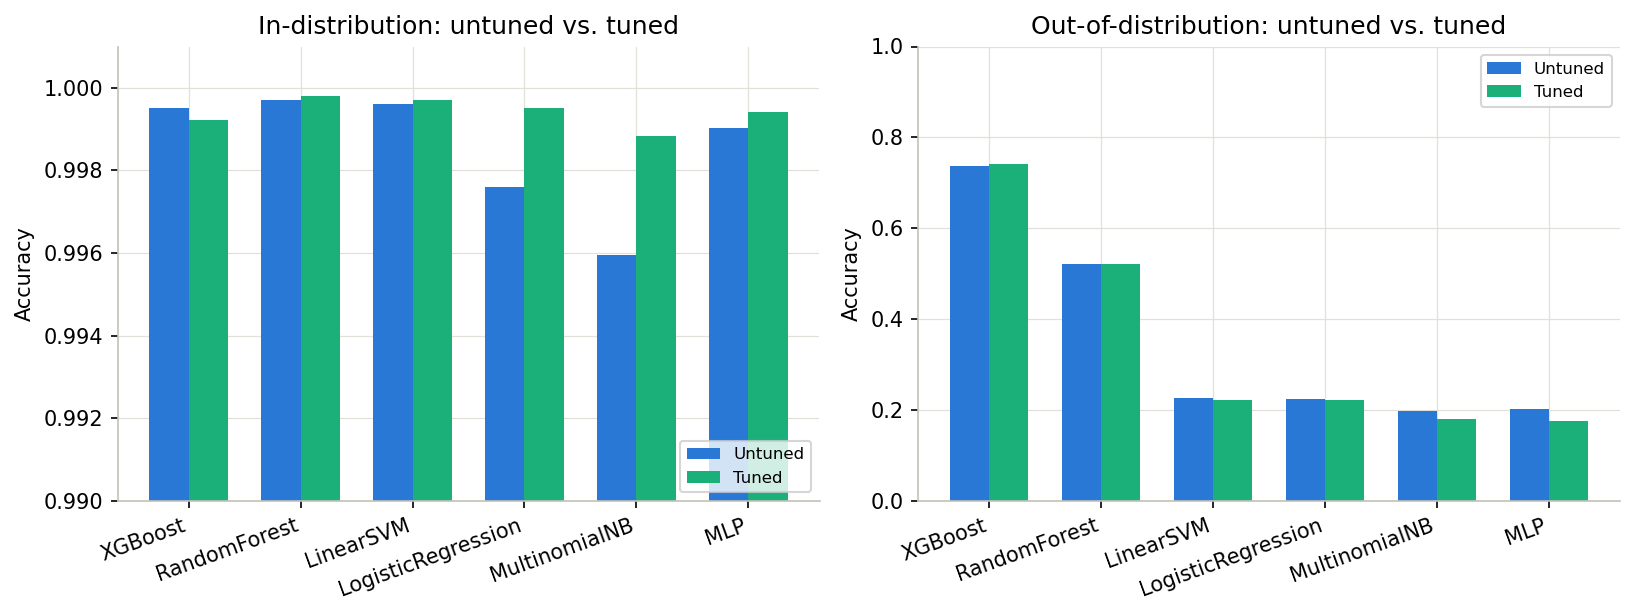
\includegraphics[width=\linewidth]{figures/hyperparameter_tuning_comparison.png}
\caption{Untuned vs.\ tuned accuracy, in-distribution (left) and OOD (right).
Tuning moves the left panel; it barely moves the right one.}
\label{fig:hyperparam}
\end{figure}

\section{Adversarial Robustness}
\label{sec:adversarial}

The OOD experiment measures robustness to natural distribution shift; it
does not test whether an attacker who knows a classifier is in place can
deliberately craft payloads to evade it, a distinct robustness axis. We
apply six black-box, non-adaptive string transforms -- the kind of
surface-level obfuscation used in practice to bypass signature-based
WAFs -- to every malicious payload in the in-distribution and OOD test
sets, and measure each of the six already-trained models' \emph{evasion
rate}: of the payloads a model correctly flagged before perturbation, what
fraction does it now miss? No retraining is performed.

\begin{itemize}
\item \textbf{Case randomization}: random per-character upper/lowercasing.
\item \textbf{Whitespace insertion}: SQL inline comments (\texttt{/**/}) or
  extra spaces at existing whitespace boundaries.
\item \textbf{URL encoding}: percent-encodes a random subset of characters.
\item \textbf{Comment injection}: inserts \texttt{/**/} between adjacent
  word characters at a low rate, a classic SQLi WAF-bypass technique.
\item \textbf{Padding dilution}: surrounds the payload with realistic
  benign filler text drawn from the training corpus (addresses, generic
  sentences), a well-known technique for evading ratio-based features.
\item \textbf{Combined}: case randomization, whitespace insertion, and URL
  encoding chained together, the strongest of the first four attacks.
\end{itemize}

\begin{figure}[!t]
\centering
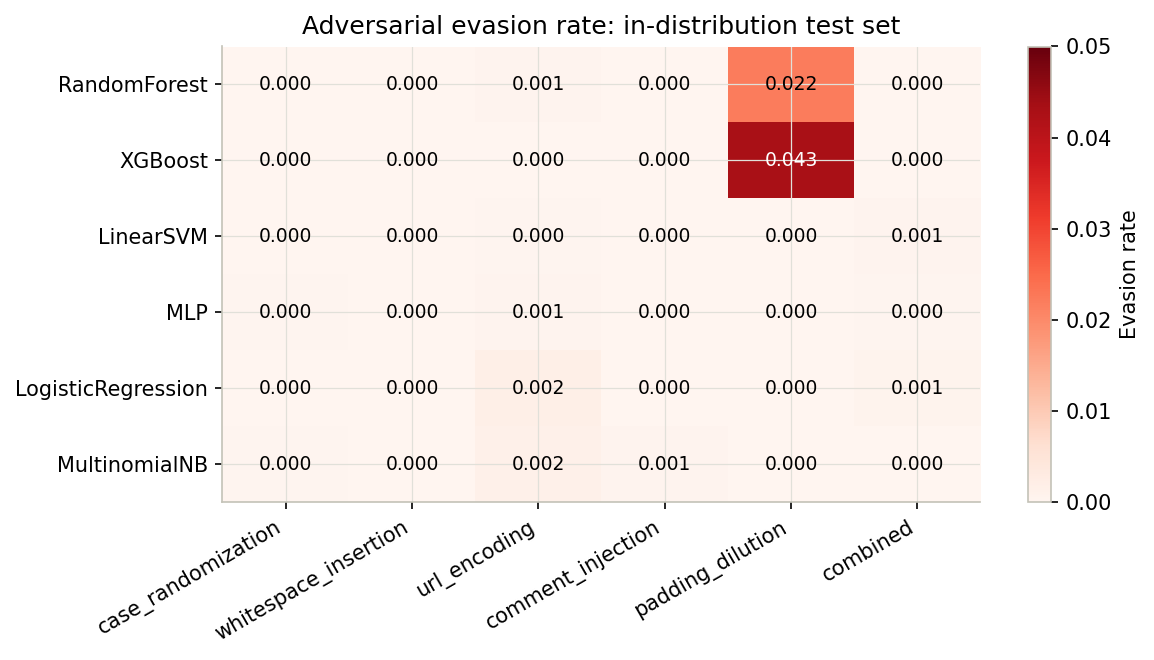
\includegraphics[width=\linewidth]{figures/adversarial_evasion_heatmap_id.png}
\caption{Evasion rate per model per transform, in-distribution test set
(3,921 malicious payloads). All cells except the padding-dilution column
for the two tree ensembles are at or near 0.000.}
\label{fig:adversarial}
\end{figure}

Figure~\ref{fig:adversarial} shows the result: \textbf{five of the six
transforms achieve near-zero evasion (0.000--0.002) against every model,
both in-distribution and OOD}. Two mechanisms explain this. First,
\texttt{TfidfVectorizer} lowercases input by default and the engineered
keyword-count features match case-insensitively, so case randomization is
fully neutralized before it reaches either representation. Second, we
verified directly that whitespace insertion, URL encoding, and comment
injection each \emph{increase} rather than decrease the engineered
features' anomaly signal on inspection: for the payload
\texttt{1' OR '1'='1}, the combined transform raises special-character
ratio from 0.417 to 0.500 and Shannon entropy from 2.355 to 3.243, pushing
the sample further from, not closer to, the benign region of feature
space.

\textbf{Padding dilution is the exception, and only against the two tree
ensembles.} It raises evasion to 2.2\% (Random Forest) and 4.3\% (XGBoost)
in-distribution, and 5.1\% and 3.1\% respectively OOD, while leaving
Logistic Regression, Multinomial NB, Linear SVM, and the MLP at 0.000 in
both settings. On the same example payload, padding dilution \emph{lowers}
special-character ratio from 0.417 to 0.051 (an 8$\times$ drop) by
lengthening the payload roughly 40-fold with benign text -- the opposite
direction from the other four transforms -- and we observed Random
Forest's predicted anomaly probability on this example fall from 0.92 to
0.53, just above its decision threshold. Tree ensembles that split on
these ratio-based engineered features appear more sensitive to dilution of
that ratio than the linear/TF-IDF-weighted models, whose per-token learned
weights are apparently less affected by added benign context at this
scale.

We emphasize what this evaluation does and does not show. It shows that
five common black-box obfuscation techniques, including several real
WAF-bypass idioms, do not meaningfully evade any of the six models, and
that a length-dilution attack achieves modest (2--5\%) evasion
specifically against tree ensembles. It does \emph{not} show general
adversarial robustness: these are non-adaptive, black-box transforms
applied uniformly, not a white-box or adaptive attacker with knowledge of
the feature extractor and decision boundary, who could plausibly design a
more targeted dilution or substitution strategy, particularly against the
tree ensembles already shown to be sensitive to it.

\section{Discussion}
\label{sec:discussion}

\textbf{Implications for ML-WAF evaluation practice.} The gap documented in
Section~\ref{sec:ood} suggests that reporting only in-distribution accuracy,
as is common practice in the literature we survey in
Section~\ref{sec:related} (and as we ourselves did in~\cite{ourprior}),
provides limited assurance about real-world deployment readiness. We
recommend that future ML-WAF papers report at minimum: (i) accuracy on a
held-out split of a second, independently sourced dataset or lexically
distinct partition where available, and (ii) macro-averaged metrics rather
than accuracy alone, given the severe class imbalance typical of attack-type
data.

\textbf{Why does the gap occur here specifically?} The lexical OOD partition
in this corpus draws its ``anomalous'' examples from different underlying
syntax templates (labeled \texttt{sql-syntax} and \texttt{js-syntax} rather
than the \texttt{sqli}/\texttt{xss} templates seen in training) while its
``normal'' examples are drawn from a different natural-language register
(informal forum/comment text vs. training's address- and numeric-field-like
normal samples). Because our TF-IDF representation is a bag of character
n-grams fit only on the training vocabulary, out-of-vocabulary
surface forms are represented purely through the engineered features and
whatever character n-grams happen to overlap -- which our ablation
(Section~\ref{sec:results-ablation}) shows are individually weaker than the
combined representation. This is consistent with XGBoost's relative OOD
strength: as the model that also ties for second-best when using engineered
features \emph{alone} (Table~\ref{tab:ablation}), it may be relying
comparatively more on the more transferable engineered signal than on
training-specific character n-grams.

\textbf{Practical deployment considerations.} Beyond accuracy, inference
latency matters for a component sitting in the request path of every HTTP
transaction. Figure~\ref{fig:latency} shows per-sample classifier latency
(excluding feature extraction) ranging from 0.0001~ms (Logistic Regression)
to 0.021~ms (Random Forest) -- all well within real-time budgets, though
Random Forest's advantage in accuracy comes with a $\sim$142$\times$ latency
and $\sim$267$\times$ model-size cost relative to Logistic Regression. Given
the OOD results, we would in fact recommend XGBoost as the more defensible
choice for a production WAF among the models tested here, trading a
negligible amount of in-distribution accuracy (99.95\% vs.\ 99.97\%) for
substantially better robustness to distribution shift (73.6\% vs.\ 52.1\%
OOD accuracy).

\begin{figure}[!t]
\centering
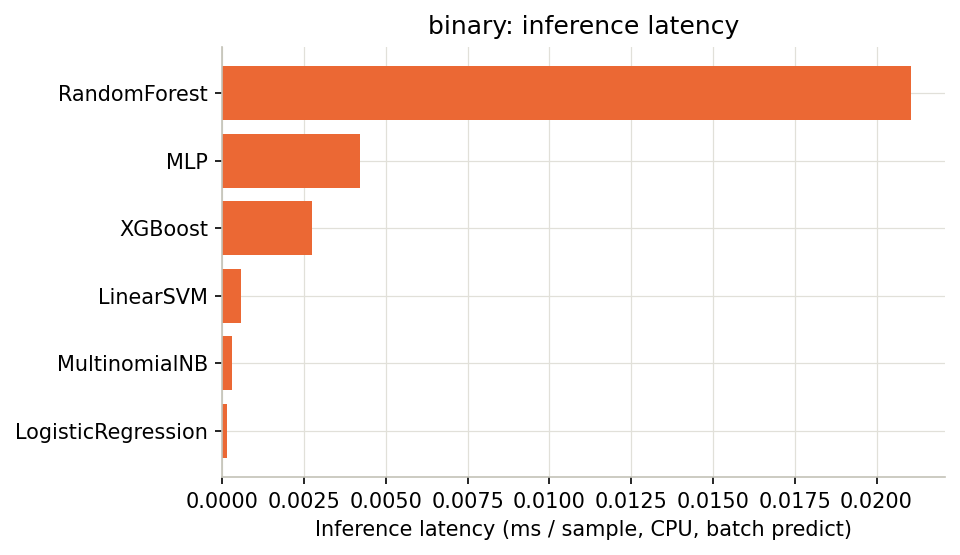
\includegraphics[width=\linewidth]{figures/binary_latency.png}
\caption{Per-sample classifier inference latency (excludes feature
extraction), binary task, sorted ascending.}
\label{fig:latency}
\end{figure}

\textbf{Limitations.} This study has several limitations. First, the OOD
partition, while lexically distinct, is drawn from the same broader corpus
and labeling methodology as the training data; a stronger test of
generalization would use a fully independent dataset (e.g., a different
public HTTP log corpus or live traffic capture), which we leave to future
work. Second, our hyperparameter search (Section~\ref{sec:hyperparam})
covers a bounded random sample of 20 configurations per model via 3-fold
CV, not an exhaustive grid or Bayesian search; a larger budget could find
different optima, though the gap's insensitivity to the search we did run
makes it unlikely a larger budget would close it. Third, our adversarial
evaluation (Section~\ref{sec:adversarial}) uses black-box, non-adaptive
string transforms representative of common WAF-bypass techniques, not a
white-box or fully adaptive attacker with knowledge of the feature
extractor and decision boundary; the tree ensembles' measurable
sensitivity to padding dilution suggests a targeted adaptive attack could
achieve higher evasion than the untargeted version tested here. Fourth,
this study only evaluates payload classification in isolation; a full WAF
deployment (e.g., our prior integration with ModSecurity, Nginx, and
Django~\cite{ourprior}) introduces additional engineering factors such as
request parsing, multi-parameter aggregation, and rule-based fallback that
are outside the present scope.

\section{Conclusion and Future Work}
\label{sec:conclusion}

We presented a controlled benchmark of six machine learning models for
WAF payload classification, combining character n-gram TF-IDF with
hand-crafted lexical features. All models achieve 99.4--99.97\% in-distribution
test accuracy, substantially exceeding the 91\% accuracy of our prior
Random-Forest-only baseline~\cite{ourprior} and confirming that engineered
lexical features and TF-IDF are complementary (feature ablation,
Section~\ref{sec:results-ablation}). Our central finding, however, is that
this near-perfect in-distribution accuracy does not transfer: on a lexically
distinct out-of-distribution test set drawn from the same corpus, accuracy
falls to 19.7--73.6\%, and the in-distribution model ranking inverts, with
XGBoost -- not the in-distribution-best Random Forest -- proving most robust.
We conclude that in-distribution accuracy, the dominant metric in the current
ML-WAF literature, is an unreliable proxy for real-world deployment
robustness, and recommend OOD or cross-corpus evaluation as a standard
reporting requirement for future work in this area. We further show that
this conclusion survives two natural objections: a randomized
hyperparameter search (Section~\ref{sec:hyperparam}) leaves the OOD gap
essentially unchanged for every model (at most $\pm$0.45 accuracy points),
ruling out under-tuning as the explanation; and a battery of six black-box
adversarial transforms (Section~\ref{sec:adversarial}) shows the trained
models are largely robust to common surface-level obfuscation (0.000--0.002
evasion for five of six transforms), with the one exception -- a
length-padding dilution attack -- achieving modest (2--5\%) evasion
specifically against the two tree-ensemble models, a concrete, testable
asymmetry future WAF designs should account for. Future work includes
evaluating against a fully independent dataset and live traffic, white-box
or adaptive adversarial evaluation targeting the tree ensembles'
demonstrated sensitivity to dilution, and extending the multi-class
analysis to additional attack families (e.g., SSRF, XXE, deserialization
attacks) as labeled data becomes available.

\section*{Reproducibility}
All code (feature engineering, training, evaluation, hyperparameter search,
adversarial testing, and figure generation), trained model artifacts, and
raw metrics produced for this paper are released alongside it. See
\texttt{code/run\_experiments.py} for the core benchmark,
\texttt{code/hyperparameter\_tuning.py} for Section~\ref{sec:hyperparam},
and \texttt{code/adversarial\_testing.py} for Section~\ref{sec:adversarial}
-- together they reproduce every number and figure in this paper from the
dataset described in Section~\ref{sec:dataset}.

\begin{thebibliography}{00}

\bibitem{owasp} OWASP Foundation, ``OWASP Top Ten,'' \url{https://owasp.org/www-project-top-ten/}, accessed 2026.

\bibitem{modsecurity} Trustwave / OWASP, ``ModSecurity: Open Source Web Application Firewall,'' \url{https://modsecurity.org/}, accessed 2026.

\bibitem{ourprior} S. U. Danish, ``Design and Implementation of a Random Forest-Based Web Application Firewall Using Open-Source Tools,'' unpublished manuscript, 2025.

\bibitem{breiman2001} L. Breiman, ``Random Forests,'' \emph{Machine Learning}, vol.\ 45, no.\ 1, pp.\ 5--32, 2001.

\bibitem{xgboost2016} T. Chen and C. Guestrin, ``XGBoost: A Scalable Tree Boosting System,'' in \emph{Proc.\ 22nd ACM SIGKDD Int.\ Conf.\ Knowledge Discovery and Data Mining (KDD)}, 2016, pp.\ 785--794.

\bibitem{salton1988} G. Salton and C. Buckley, ``Term-Weighting Approaches in Automatic Text Retrieval,'' \emph{Information Processing \& Management}, vol.\ 24, no.\ 5, pp.\ 513--523, 1988.

\bibitem{httpparamsdataset} Morzeux, ``HttpParamsDataset,'' GitHub repository, \url{https://github.com/Morzeux/HttpParamsDataset}, accessed 2026.

\end{thebibliography}

\end{document}
